\chapter{General Discussion}

This chapter concludes my thesis by summarising the key findings and implications of our results in light of the existing literature on transcriptional variation in AD and the current status of long-read sequencing approaches for transcriptome profiling. This discussion will also summarise some of the key limitations and caveats that should be considered when interpreting our results. Finally, this chapters concludes by giving an outline of the future directions of the research presented in this thesis.       

\section{Key findings}
I hypothesised that transcriptional regulation, particularly alternative splicing, is dysregulated in the development of AD pathology. However, previous studies investigating splicing and transcript-level expression variations have been constrained by inherent limitations of short-read RNA-Seq approaches. The primary aim of this thesis was to address these limitations and leverage the power of novel long-read sequencing technologies to accurately characterise the transcriptomic landscape in a mouse model of AD, with a particular focus on identifying splicing patterns associated with the progression of tau pathology.

In meeting the objectives set out in \textbf{Chapter 1}, we:
\begin{itemize}
	\item optimised a novel laboratory workflow and bioinformatics pipeline in \textbf{Chapter 3} to profile full-length transcripts using two state-of-the-art, long-read sequencing approaches: PacBio isoform sequencing (Iso-Seq) and ONT nanopore cDNA sequencing.  
	
	\item characterised the global transcriptome landscape of the mouse cortex using Iso-Seq in \textbf{Chapter 4}, revealing widespread cortical isoform diversity and extensive usage of alternative splicing events. 
	
	\item identified transcriptional and splicing alterations associated with the progression of tau pathology in rTg4510 mice in \textbf{Chapter 5}, finding evidence for profound isoform switching events in genes previously implicated in AD. 
	
	\item performed long-read targeted sequencing of 20 AD-risk genes in \textbf{Chapter 6}, identifying robust transcript expression differences in microglial-specific genes associated with tau accumulation in rTg4510 mice.    
\end{itemize}

\section{Implications and limitations}

\subsubsection{Incomplete reference annotations with detection of novel isoforms} 
One of the common overarching themes in our long-read sequencing analyses - and those recently published by others - is the extensive detection of novel isoforms not present in current reference annotations, highlighting the constraints of previous transcriptome studies to accurately study the regulation of alternative splicing. Global transcriptome profiling of the mouse cortex (\textbf{Chapter 4}) detected over 20,000 novel isoforms, with evidence of novel splice junctions and splicing events. The power to discover more novel and rare isoforms with long-read sequencing is highlighted in our target enrichment of AD-associated genes (\textbf{Chapter 6}), with over 2000 novel isoforms annotated to \textit{Apoe} alone. Given that genetic and transcriptomic studies are fundamentally reliant on accurate gene annotations, this "incompleteness" of existing annotations limits our understanding of the role of transcriptional variation in complex diseases. Of note, a recent study found that genes associated with neurodegenerative disorders, \textit{SNCA, APOE} and \textit{CLU} (also included in the target gene list), were significantly under-represented in the human reference annotations after leveraging transcriptome data from the GTEx consortium\cite{Zhang2020b}.  

We envisage that the number of novel isoforms detected will continue to grow with advances in sequencing technologies. However, one of the major challenges in long-read sequencing is how to best assess the validity and quality of these isoforms. Despite the capacity to enrich for full-length transcripts, the standard long-read sequencing protocol is still reliant on cDNA synthesis and PCR amplification, creating artefacts that can be misinterpreted as novel isoforms generated from non-canonical splicing. RNA degradation can also result in isoforms with incomplete 5'ends resulting in misinterpretation of these artefacts as novel isoforms with novel alternative initiation start sites\cite{Kuo2020}. Of note, we found that more than 98\% of our ONT novel transcripts had one read across two samples. While we are confident about the validity of our transcriptome annotations - i.e. we undertook stringent filtering and cross-validated isoforms using two independent long-read sequencing approaches - it will be important to undertake further experimental validation and integrate with other functional data. 

\subsubsection{Functional importance of RNA isoforms on proteome diversity} 
As we (and others) have shown, the high-throughput sequencing of full-length transcripts highlights the widespread isoform diversification through alternative splicing of the transcriptome. However, large-scale proteomic studies have failed to recapitulate this isoform diversity at the protein level, sparking fierce debate about the impact of alternative splicing on protein production and function\cite{Tress2017a,Blencowe2017,Tress2017b}. This disparity is likely to be driven by the poor sensitivity and incompleteness of current protein reference databases, limiting its utility for isoform-based analyses\cite{Reixachs-Sole2022}. Notably, recent studies using "long-read proteogenomics" - an integrative approach that incorporates ORF annotations derived from long-read sequencing data with peptides detected using mass-spectrometry (MS) - revealed hundreds of protein isoforms undetectable using traditional MS \cite{Miller2022,Wang2019a}. This approach further allowed identification of novel peptides that corresponded to novel exons and splicing events derived from improved long-read annotations\cite{Miller2022,KayLeung2021}.  

We show that the isoform landscape for the majority of AD-risk genes characterised in this thesis were dominated by a few major isoforms (\textbf{Chapter 6}). This raises questions about how functionally important these alternatively-spliced novel isoforms are, particularly when they only differ slightly from the major isoforms. However, we know that minor changes in the open reading frame, while not inducing large protein conformational changes, can disrupt post-translational modifications and impact protein function\cite{Reixachs-Sole2022}. This is supported by identification of \textit{TREM2} variants known to impact ligand binding and modulate downstream signalling pathways, while broadly maintaining protein structure and stability\cite{Kober2016}. Furthermore changes in the 5' and 3' UTR, while resulting in no observable effect on the protein product, can affect transcript stability, export, localisation and translation efficiency\cite{Reixachs-Sole2022}. Finally, it is possible that the additive effects resulting from the expression of multiple low-abundant, but mis-spiced isoforms could have global deleterious impacts by: i) altering the ratio of canonical isoforms, ii) overwhelming the ubiquitin-proteasome pathway with accumulation of nonsense-mediated decay polypeptides, and iii) generating insoluble protein aggregates, which underlie the neuropathology of AD and other neurodegenerative diseases\cite{Davis2018}.

\subsubsection{Understanding the development of tau pathology through transcriptome profiling}
In providing a "snapshot" of the cellular state, transcriptome profiling can provide key insights into the mechanisms underlying disease changes, enabling the elucidation of key pathogenic pathways. My experiments also included the profiling of the cortex across multiple time-points (2, 4, 6 and 8 months) spanning the development of tau pathology in the rTg4510 mouse model (\textbf{Chapter 5, 6}), further allowing us to evaluate temporal transcriptional changes. In line with findings from RNA-Seq studies using other mouse models, we found widespread transcriptional differences associated with tau accumulation (\textbf{Chapter 5}). Furthermore, our long-read sequencing datasets were powered to identify robust differences in isoform expression, which drove gene expression alterations that were well established in the development of human AD (\textbf{Chapter 5, 6}). Highlighting the utility of isoform-level analyses, we also identified a number of genes presented with differential isoform usage and isoform switches without overall gene-level expression differences, particularly at the later stages of tau pathology. Characterisation of these alternatively-spliced isoforms suggest these alterations could have functional biological consequences, though more work will be needed to confirm this.   

\subsubsection{Cellular heterogeneity in isoform diversity in the brain}
Alternative splicing is known to define tissue-specificity, with more than a third of human genes found to express tissue-dominant isoforms and is characterised by tissue-specific splicing events\cite{Wang2008,Yeo2004}. Recent studies using single-cell sequencing further support the evidence for cell-type-specific splicing, particularly in the brain where it plays an important role in neuronal development and maintenance.

However, the vast majority of AD transcriptome profiling studies, including the studies presented in this thesis, have been limited to analyses on "bulk" tissue comprised of a complex mix of different cell-types. We were therefore unable to draw conclusions about cell-specific splicing variations, despite recent studies reporting differential expression of cell-specific \textit{BIN1} isoforms in the AD brain. Furthermore, given AD pathogenesis is characterised with progressive changes in cell composition that vary across different brain regions, it becomes more challenging to disentangle tissue and cell-specific AD-associated variants. Having not accounted for cellular heterogeneity in our studies, we acknowledge that our results may be a partial reflection of microgliosis and neuronal loss. While this challenge can be addressed using a combined approach of single-cell sequencing and long-read sequencing, as shown in recent studies (reviewed in \cref{tab: longread_advancedstudies}), this strategy is currently limited to achieve the depth required to detect reliable disease- and cell-specific splicing variations. 

\subsubsection{Translational relevance of AD mouse models}
One of the key challenges of studying transcriptomic variation in human post-mortem brain tissue is that they typically represent the end-stage of the disease, thus limiting the detection of progressive disease-associated variations and the ability to infer causality. Although mouse models act as valuable reductionist tools to dissect the processes that drive the onset and progression of AD pathology, there are some concerns about how representative they are of sporadic, late-onset AD in human. The integration of the calcium-calmodulin kinase IIa promoter (CaMKIIα-tTA) and human \textit{MAPT} transgenes in the rTg4510 mouse model have also been found to disrupt the expression of five endogenous mouse genes (\textit{Vipr2}, \textit{Wdr60}, \textit{Esyt2}, \textit{Ncapg2} and \textit{Ptprn2}, which may contribute to the neurodegenerative phenotype observed in these mice\cite{Castanho2020,Gamache2019}. Although we have identified transcriptional differences that broadly overlapped with previous transcriptome studies on human post-mortem brain tissue - including \textit{Gfap} upregulation and \textit{Bin1} differential isoform expression - future work will be essential to perform cross-species analyses and translate our findings to human.      
	
\section{Future directions}
In this thesis, I have presented an optimised laboratory and bioinformatics pipeline, a set of empirical findings, and a comprehensive resource, which serve to deepen our understanding of isoform diversity in the cortex and the role this plays in the development of AD pathology. However, as discussed above, the findings presented are not without limitations inherent to the research question and methods chosen. As such, the following section details a number of future directions proposed to address these limitations and foster additional research in this area.   

\subsubsection{Integration with other datasets} 
As described in \cref{intro:AS}, alternative splicing is highly regulated in a concerted manner requiring multiple mechanistic components, including epigenetic modifications such as DNA methylation and histone modifications. Epigenetics refers to the heritable, but reversible, alterations to the chromatin structure that have been shown to influence splicing through the recruitment of splicing factors\cite{Yang2014, Shukla2011, Zhang2020a, Shukla2011, Luco2011}. A number of studies, for example, have shown that gene body DNA methylation can influence polymerase processivity and elongation rate, which can in turn determine the splicing of weak alternative exons \cite{Yang2014, Shukla2011}. Integrating our transcriptomic dataset with epigenetic data (DNA methylation and histone modifications) generated on the same mouse samples (Castanho et al., unpublished data, 2022) would be important to further understand the mechanisms driving transcriptional regulation in AD development and provide insights into the cross-talk between splicing and epigenetics. 

One of the key limitations of our analyses is that they were performed on "bulk" tissue, limiting the detection of cell-specific isoforms and meaning that some of our results could be confounded by cellular heterogeneity. Moving forward, mouse single-cell data derived from isolating specific cell populations - using methods such as fluorescence-activated cell sorting (FACS) (Policicchio  et al., unpublished data, 2022) - or publicly available mouse single cell RNA-Seq datasets could be used to infer cell populations in our dataset with the potential to assess cell-type specific splicing events.   

\subsubsection{Experimental and functional validation}
Although we used ONT nanopore sequencing and short-read RNA-Seq to validate and complement our Iso-Seq data with notable success (\textbf{Chapter 6}), further experimental validation of the novel isoforms and empirical findings presented in this thesis is important. This could be achieved using a number of molecular biology techniques, such as i) RT-qPCR with primers that flank the alternatively-spliced region, ii) western blot and enzyme-linked immunosorbent assays (ELISA) to identify protein isoforms, and iii) fluorescence \textit{in-situ} hybridisation (FISH) and immunohistochemistry techniques for isoform visualisation at the RNA and protein level, respectively. Of note, all these methods require specific primers and antibodies that are unique to the isoform of interest. Finally, the functional consequences of alternative splicing events can be explored using various assays, such as CRISPR/Cas9 system and minigene splicing reporters among others, to accurately and rapidly recapitulate splicing effects in cultured cells.  


\subsubsection{Transcriptome profiling of human post-mortem brain tissues}  
Ultimately, the utility of animal models is to translate and recapitulate findings to humans. Consequently, the findings presented in this thesis provide the foundation for a broader follow-up study in human post-mortem brain tissues. While this is beyond the scope of my written thesis, as part of this research I performed targeted Iso-Seq of 20 AD risk-genes in a subset of prefrontal cortex samples from the Brains for Dementia Research (BDR) cohort (n = 15 controls, 15 AD cases). In applying the same sequencing approach and bioinformatics pipeline described in \textbf{Chapter 6}, preliminary analyses highlight widespread detection of novel isoforms annotated to AD-risk genes (\cref{fig:adbdr}\textbf{A}), characterised with extensive usage of alternative splicing events (\cref{fig:adbdr}\textbf{B}). Following a more detailed mapping of the isoform landscape, future work will involve a comprehensive case-control analyses at the transcript-level and compare findings from the tau mouse model. Furthermore, we have applied other profiling approaches - such as genomic profiling (ATAC sequencing), epigenetics (DNA and histone modifications), transcriptomics (RNA-Seq, miRNA) and proteomics (mass-spectrometry) - on the same samples, enabling a comprehensive integrated multi-omics approach to gain deeper mechanistic insights into the development of AD pathogenesis.     

\begin{landscape}
	\begin{figure}[!htp]
		\centering
		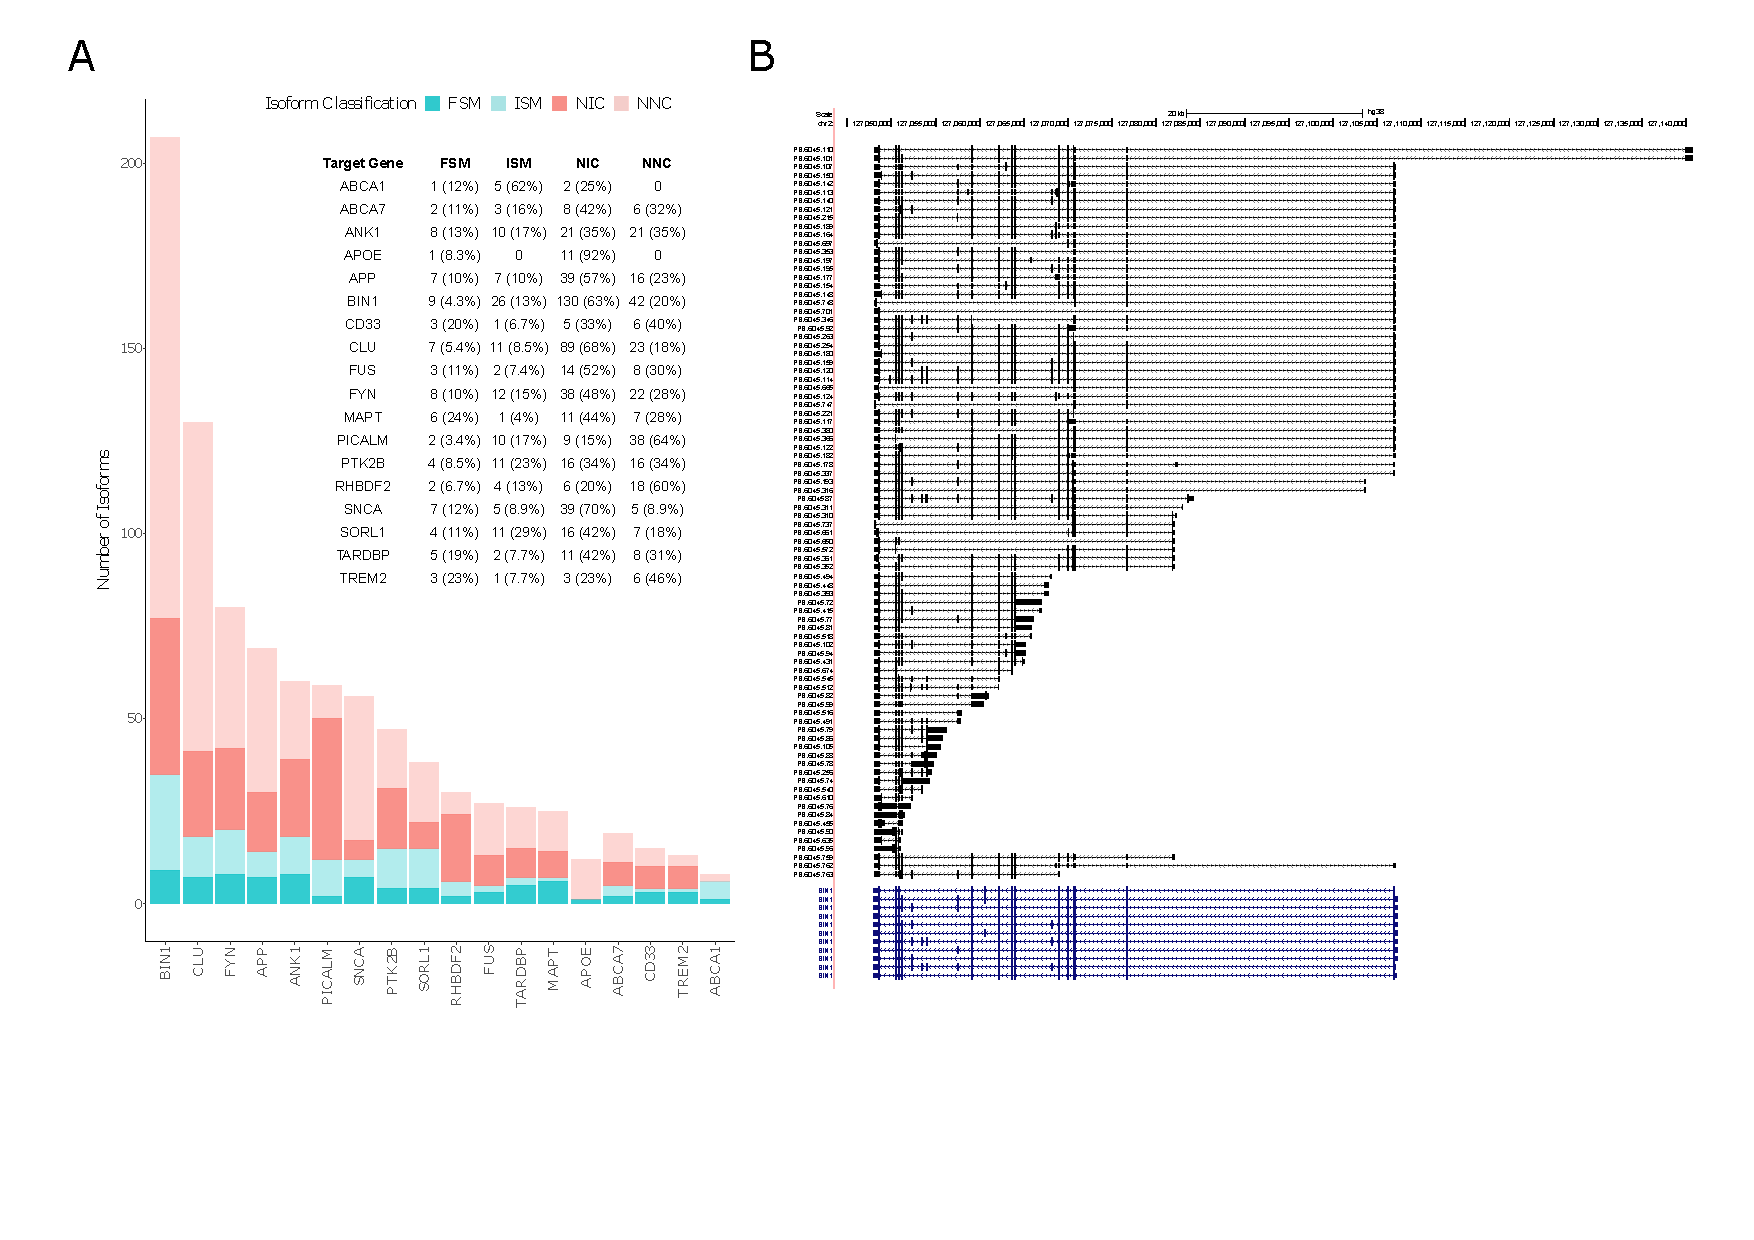
\includegraphics[page=1,trim={1.5cm 3.5cm 2cm 1cm}, scale = 0.85]{Figures/Bin1_ADBDR.pdf}
		\captionsetup{width=1.5\textwidth}
		\caption[Preliminary results from targeted profiling of human post-mortem brain tissue]%
		{\textbf{Widespread detection of novel isoforms annotated to AD-risk genes from targeted profiling of AD human post-mortem brain tissue.} Shown are some preliminary results, showing \textbf{(A)} the number of known (FSM, ISM) and novel isoforms (NIC, NNC) annotated to AD-risk genes, classified using \textit{SQANTI} (detailed in \cref{section: sqanti_annotations}), and \textbf{(B)} a UCSC genome browser track of a a subset of isoforms annotated to \textit{BIN1} after Iso-Seq targeted profiling of AD human post-mortem brain tissue. The same Iso-Seq targeted laboratory workflow and bioinformatics pipeline, as that optimised for the mouse cortex in \textbf{Chapter 6}, was applied. Iso-Seq-derived isoform annotations and human reference annotations (hg38, GENCODE) are in black and blue, respectively.}   
		\label{fig:adbdr}
	\end{figure}	
\end{landscape}   

\section{Conclusion}
Taken altogether, my thesis harnessed the power of long-read sequencing to extend our understanding of the mouse cortical transcriptome and assess splicing variation associated with the development of tau pathology in a transgenic mouse model. To our knowledge, it is the first study to profile a mouse model of AD pathology, rTg4510, using both PacBio Iso-Seq and ONT nanopore sequencing. In providing a framework for the comprehensive characterisation of the AD isoform landscape at a global and targeted level, we revealed unprecedented diversity of alternatively-spliced isoforms annotated to AD-risk genes. We identified widespread transcriptional and splicing variations paralleling the development of tau pathology, with evidence of differential isoform expression and usage. Our findings corroborated data from previous studies implicating a role for altered splicing and immune response in the development of AD pathology. The data presented in this thesis provides a strong foundation for characterising the transcriptomic landscape in the human AD brain and represents a valuable resource to the research community.   